\Answer{}
Since we already have the electrostatic field \(\bm{\phi}\) from Problem~\ref{sec:pe},
we now need to add it to the differential operator (the discrete Laplacian).
Equation~\eqref{eq:del2phi} is now rewritten as
%
\begin{multline}\label{eq:del2psi}
    \bigl(-\nabla^2 + q \phi\bigr) \psi(x, y) =
    \frac{ 1 }{ a^2 } \bigl(\psi(x - a, y) - 2 \psi(x, y) + \psi(x + a, y)\bigr) +\\
    \frac{ 1 }{ a^2 } \bigl(\psi(x, y - a) - 2 \psi(x, y) + \psi(x, y + a)\bigr) +
    q \phi(x, y) \psi(x, y).
\end{multline}
%
As stated in Problem~\ref{sec:pe},
$\phi(x, y)$ can be reshaped as an \(N^2 \times 1\) vector,
which can fit into the diagonal of the \(N^2 \times N^2\) Laplacian matrix.

Since the Hamiltonian is a Hermitian matrix, we could use the Lanczos algorithm to
solve its eigenvalues and eigenvectors.
The input of our algorithm is the symmetric matrix
%
\begin{equation}\label{eq:hamiltonian}
    \hat{H} = -\nabla^2 + q \phi
\end{equation}
%
where \(\phi\) is the reshaped matrix from the electrostatic potential \(\bm{\phi}\).
We also need a small number ($k$) of iterations (\(30\) here).

The procedure is as follows:
%
\begin{enumerate}
    \item\label{it:v1} Let $\bm{v}_1 \in \mathbb{ R }^n$ be an arbitrary vector with Euclidean norm $1$.
    \item Let $\bm{w}'_1 = \mathrm{A} \bm{v}_1$, and
          $\alpha_1 = \bm{w}^{\prime\intercal}_1 \cdot \bm{v}_1 = \bm{v}_1^\intercal \mathrm{A} \bm{v}_1$,
          and $\bm{w}_1 = \bm{w}'_1 - \alpha_1 \bm{v}_1$.
    \item For $j = 2$, $\ldots$, $k$, where $k$ is the maximum number of iterations, do
          \begin{enumerate}
              \item Let $\beta_j = \| \bm{w}_{j-1} \|$.
              \item If $\beta_j \neq 0$, then let $\bm{v}_j = \bm{w}_{j-1} / \beta_j$.
              \item Let $\bm{w}'_j = \mathrm{A} \bm{v}_j$, and
                    $\alpha_j = \bm{w}^{\prime\intercal}_j \cdot \bm{v}_j = \bm{v}_j^\intercal \mathrm{A} \bm{v}_j$,
                    and $\bm{w}_j = \bm{w}'_j - \alpha_j \bm{v}_j$.
          \end{enumerate}
    \item Juxtapose all the $\bm{v}_j$s as the
          column vectors of a $N^2 \times k$ matrix $\mathrm{V}$.
          Form a tridiagonal matrix $T_k$ using $\{\alpha_j\}$ and $\{\beta_j\}$.
\end{enumerate}
%
The relation between $\mathrm{A}$, $\mathrm{T}$, and $\mathrm{V}$ are
%
\begin{align}
    \mathrm{T} & = \mathrm{V}^\intercal \mathrm{A} \mathrm{V}, \\
    \mathrm{A} & = \mathrm{V} \mathrm{T} \mathrm{V}^\intercal.
\end{align}
%
That is, $\mathrm{V}$ can tridiagonalize $\mathrm{A}$.
We could use other programs to further diagonalize the tridiagonal matrix $\mathrm{T}$,
which is much simpler than diagonalizing $\mathrm{A}$ from the beginning.

If $\lambda$ is an eigenvalue of $\mathrm{A}$, and if $\mathrm{T}\bm{w} = \lambda \bm{w}$
($\bm{w}$ is an eigenvector of $\mathrm{T}$), then
%
\begin{equation}\label{eq:eigen}
    \bm{v}' = \mathrm{V} \bm{w}
\end{equation}
%
is the corresponding eigenvector of $\mathrm{A}$. Namely, if we know the eigenvector
of $\mathrm{T}$, then it is easy to solve the eigenvector of $\mathrm{A}$.

Therefore, we could understand the idea of restarting.
Equation~\eqref{eq:restart} is an index notation rewriting of Equation~\eqref{eq:eigen}.
After \(k\) steps of the Lanczos iterations, we obtain a $k \times k$ tridiagonal matrix
$\mathrm{T}$ and $k$ Lanczos vectors (each of which has the length
of the full system).
These $k$ Lanczos vectors span a $k$-dimensional Krylov subspace in the full space.
We will use $\bm{w}$, the eigenvector of $\mathrm{T}$, to recover an approximate
eigenvector of $\mathrm{A}$. And use this new ``eigenvector'' as our initial value
for the Lanczos iterations Step~\ref{it:v1} instead of a random vector.
Repeat this procedure for $30$ to $40$ times, and use the last recovered
eigenvector $\bm{v}$ of matrix $\mathrm{A}$ as our final solution.

The code for a \code{maxiter} steps of Lanczos iterations is shown in
Snippet~\ref{lst:lanczos}. The returned values are a symmetric tridiagonal matrix
\code{T} and a matrix \code{V} storing those Lanczos vectors.

\begin{algorithm}[!hbt]
    \caption{The Lanczos algorithm implementation of solving
        \(\mathrm{ A }\bm{ x } = \lambda\bm{ x }\), with at most \code{maxiter}
        iterations.}
    \label{lst:lanczos}
    \begin{juliacode}
function lanczos(A::AbstractMatrix, 𝐯₁=rand(size(A, 1)); maxiter=30)
    n = 1  # Initial step
    𝐯₁ = normalize(𝐯₁)
    V = Matrix{eltype(𝐯₁)}(undef, length(𝐯₁), maxiter)
    V[:, n] = 𝐯₁
    𝐰′₁ = A * 𝐯₁
    α₁ = 𝐰′₁ ⋅ 𝐯₁
    𝐰ₙ = 𝐰′₁ - α₁ * 𝐯₁  # 𝐰₁
    𝛂 = Vector{eltype(float(α₁))}(undef, maxiter)
    𝛃 = Vector{Float64}(undef, maxiter)
    𝛂[n], 𝛃[n] = α₁, 0
    for n in 2:maxiter
        𝐰ₙ₋₁ = 𝐰ₙ
        𝛃[n] = norm(𝐰ₙ₋₁)
        if !iszero(𝛃[n])
            𝐯ₙ = 𝐰ₙ₋₁ / 𝛃[n]
            V[:, n] = 𝐯ₙ
        end
        𝐰′ₙ = A * 𝐯ₙ
        𝛂[n] = 𝐰′ₙ ⋅ 𝐯ₙ
        𝐰ₙ = 𝐰′ₙ - 𝛂[n] * 𝐯ₙ - 𝛃[n] * V[:, n - 1]
    end
    T = SymTridiagonal(𝛂, 𝛃[2:end])
    return T, V
end
    \end{juliacode}
\end{algorithm}

The code for finding the eigenvector of the matrix $\mathrm{A}$ is shown in
Snippet~\ref{lst:restart}, where function \code{recover_eigvec} corresponds to
Equation~\eqref{eq:eigen}, and we use Julia's \code{eigen} function to find the eigenvalues
and eigenvectors of $\mathrm{T}$. Since we want to see the ground state, we focus on the
eigenvalue corresponding to the lowest energy. Since all the eigenvalues are positive in our
problem, we could use function \code{argmin} to find the index of the smallest eigenvalue.
This is necessary because the returned eigenvalues may not have been sorted.

We repeat the procedures in Snippet~\ref{lst:lanczos} and Snippet~\ref{lst:restart}
for $30$ to $40$ times, and the last eigenvector we produced is the desired eigenvector
of our system \eqref{eq:hamiltonian}.

\begin{algorithm}[!hbt]
    \caption{The algorithm for finding the eigenvectors of the matrix $\mathrm{T}$
        and $\mathrm{A}$ as our next initial value.}
    \label{lst:restart}
    \begin{juliacode}
recover_eigvec(V, 𝐰) = normalize(V * 𝐰)

function restart_lanczos(T, V)
    vals, vecs = eigen(T)
    index = if all(vals .> 0)
        argmin(vals)  # Index of the smallest eigenvalue
    else
        argmax(abs.(vals))  # Index of the smallest eigenvalue
    end
    𝐰 = vecs[:, index]  # Associated eigenvector
    return recover_eigvec(V, 𝐰)
end
    \end{juliacode}
\end{algorithm}

However, as in Problem~\ref{sec:pe}, we still need to correctly set our boundary
conditions. In this problem, they are slightly simpler since the wave function
in the internal square is also zero.

Look into the \code{lanczos} function, which we do the actual iterations on
the hamiltonian.
First, we need to set $\bm{v}_1$ and $\bm{w}'_1$ to be zero on the boundary of the region
and in the internal square. Remember to apply these conditions first before
normalizing $\bm{v}_1$. With $\bm{v}_1$ and $\bm{w}'_1$ set, $\bm{w}_1$ within these
regions are automatically zero since
%
\begin{equation}
    \bm{w}_1 = \bm{w}'_1 - \alpha_1 \bm{v}_1.
\end{equation}
%
Then within each Lanczos iteration, we also set $\bm{w}'_n$ to be zero in these regions,
too. But we do not need to apply these conditions to $\bm{v}_n$,
since $\bm{v}_n$ is just normalized $\bm{w}_{n-1}$, which is always zero
in the aforementioned areas.

We plot the heatmap and the manifold of our eigenvector, $\bm{\psi}$, in
Figure~\ref{fig:psi_heatmap} and Figure~\ref{fig:psi_surface}, respectively.
As we can see, it is indeed zero in the specified areas, as expected.
$\bm{\psi}$ is thusly the ground state of the system \eqref{eq:hamiltonian}.
The basis of this wave function is each point on the grid, and the coefficients
in the eigenvector are the $z$-coordinates shown in the figures.

\begin{figure}[!hbt]
    \centering
    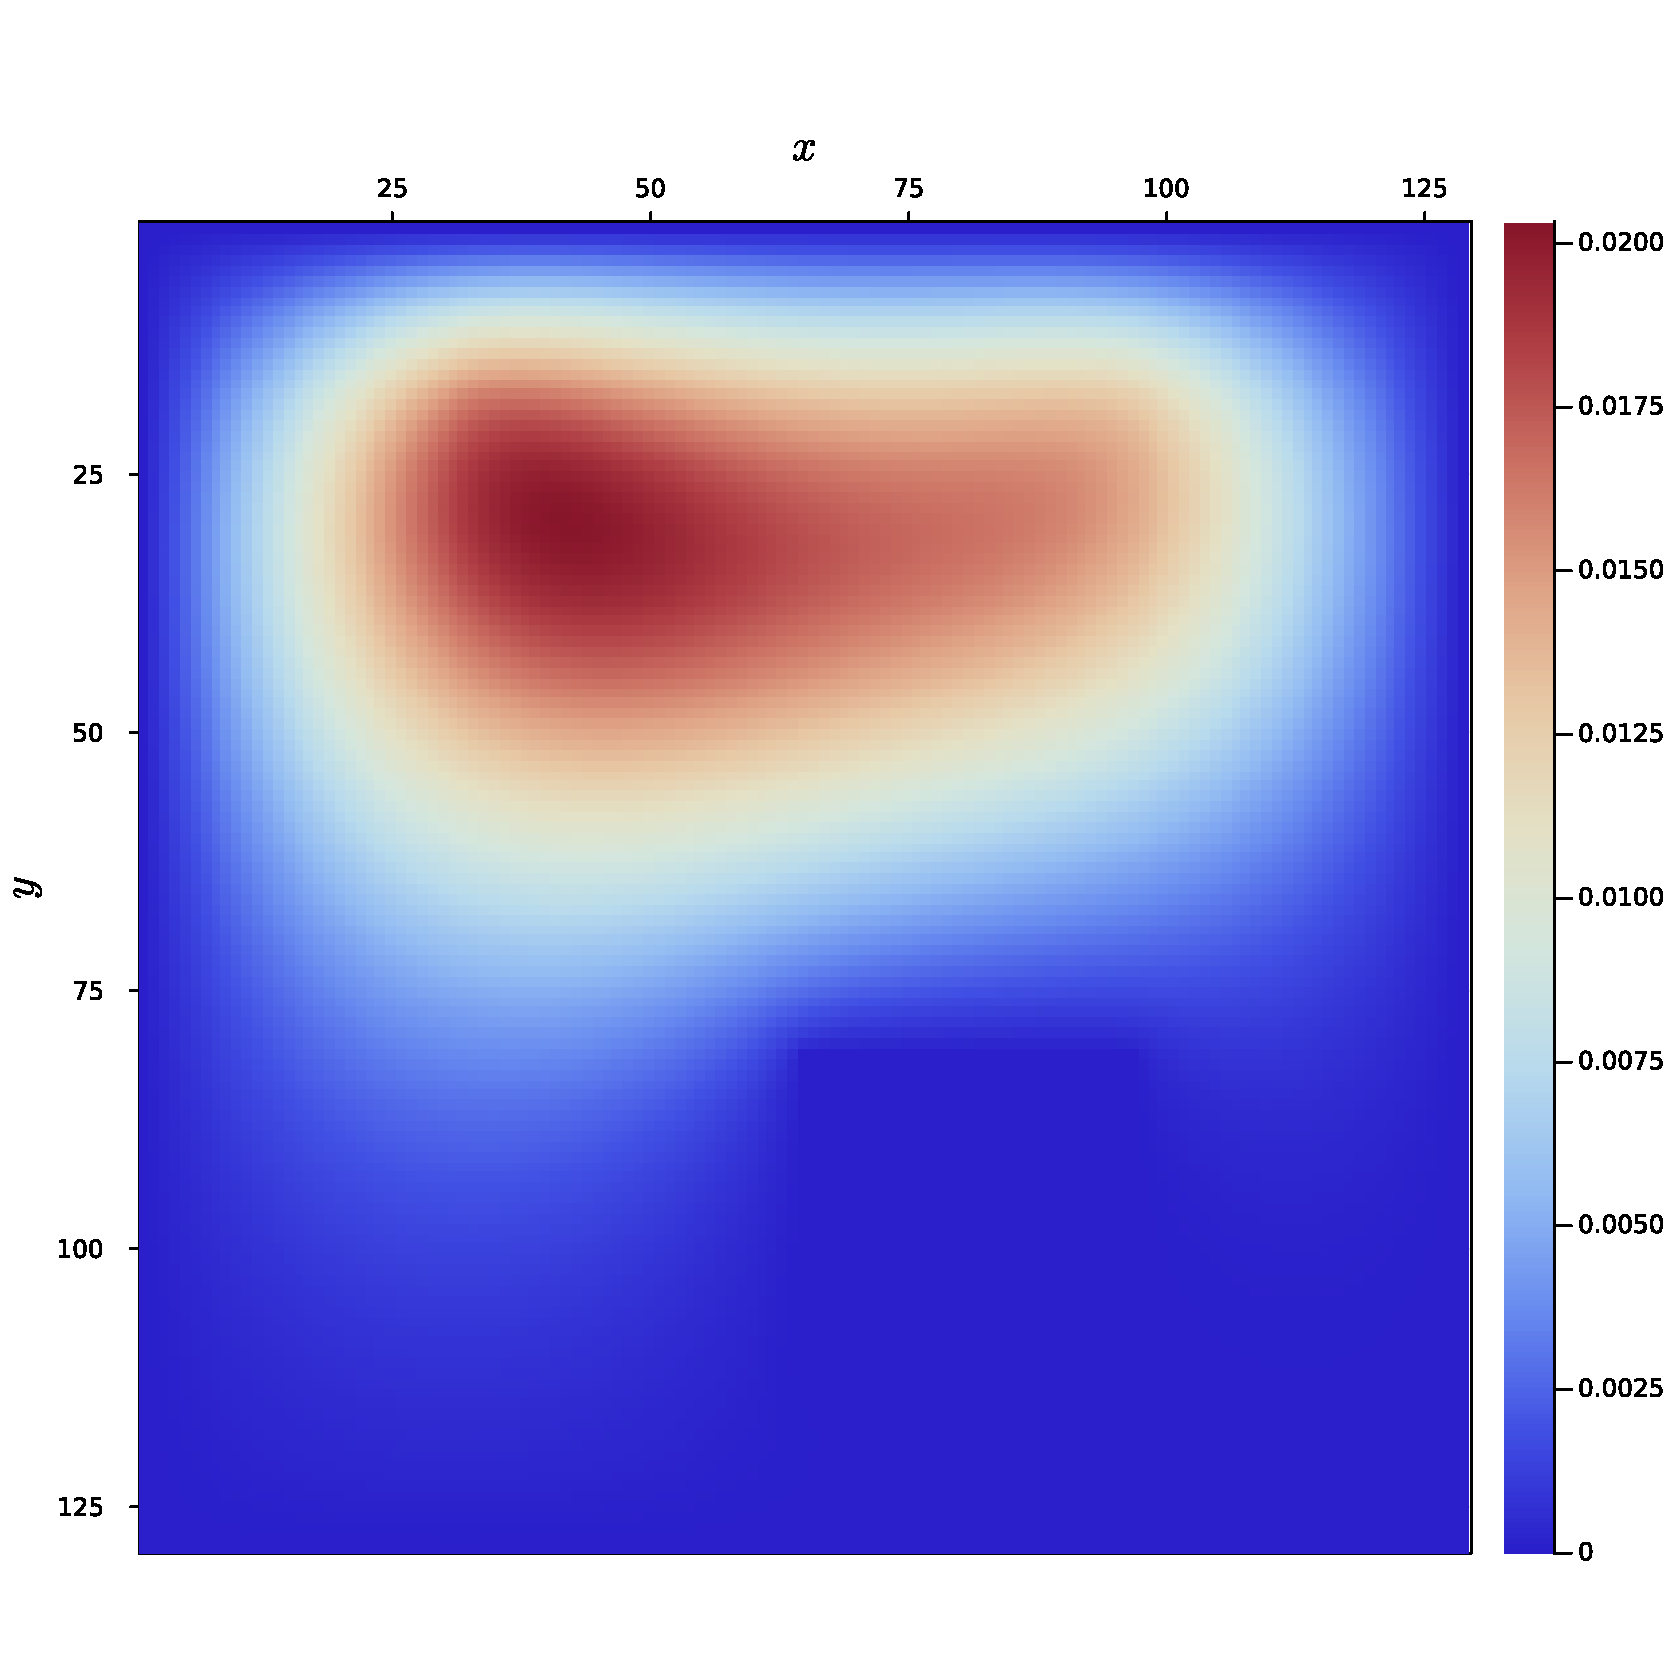
\includegraphics[width=0.8\textwidth]{psi_heatmap}
    \caption{The heatmap of the final wave function, which corresponds to the
        lowest energy $E_0$ of the system.}
    \label{fig:psi_heatmap}
\end{figure}

\begin{figure}[!hbt]
    \centering
    \includegraphics[width=0.8\textwidth]{psi_surface}
    \caption{The surface plot of the final wave function, which corresponds to the
        lowest energy $E_0$ of the system.}
    \label{fig:psi_surface}
\end{figure}

However, the physical meaning of the wave function is marginal.
What is more important is the probability implied by the wave function.
The probability of the charged particle appearing at position $x$ is defined by
%
\begin{equation}
    P(x) = \abs{\psi(x)}^2 = \psi^\ast(x) \psi(x).
\end{equation}
%
And the probability that its position $x$ will be in the interval $a \leq x \leq b$ is the
integral of the density over this interval:
%
\begin{equation}\label{eq:Prange}
    P(a \leq x \leq b) = \int_{a}^{b} \abs{\psi(x)}^2 \, \mathrm{d}x.
\end{equation}
%
We will use this equation later.

We plot the probability of the charged particle appearing at any position
as a heatmap and a surface plot in Figure~\ref{fig:P_heatmap} and Figure~\ref{fig:P_surface},
respectively.
Clearly, they show that the charged particle is not possible to be present in the
internal square and on the boundary.
They also indicate that the particle is more likely to be found near the negative
point charge located at \((0.25L, 0.125L)\). Because there is a positive potential
$\phi = 5$ near the negative charge at \((0.75L, 0.125L)\), where the former partially
screens the latter's attraction force and drives the positive-charged particle away.
We can prove this by testing the possibility of the particle appearing in the
range where $y < 0.5L$ using Equation~\eqref{eq:Prange}, the result is
%
\begin{equation}
    P(x, y < 0.5L) \approx 0.966264.
\end{equation}
%
Therefore, the particle dominantly will be found in the area where $y < 0.5L$.

\begin{figure}[!hbt]
    \centering
    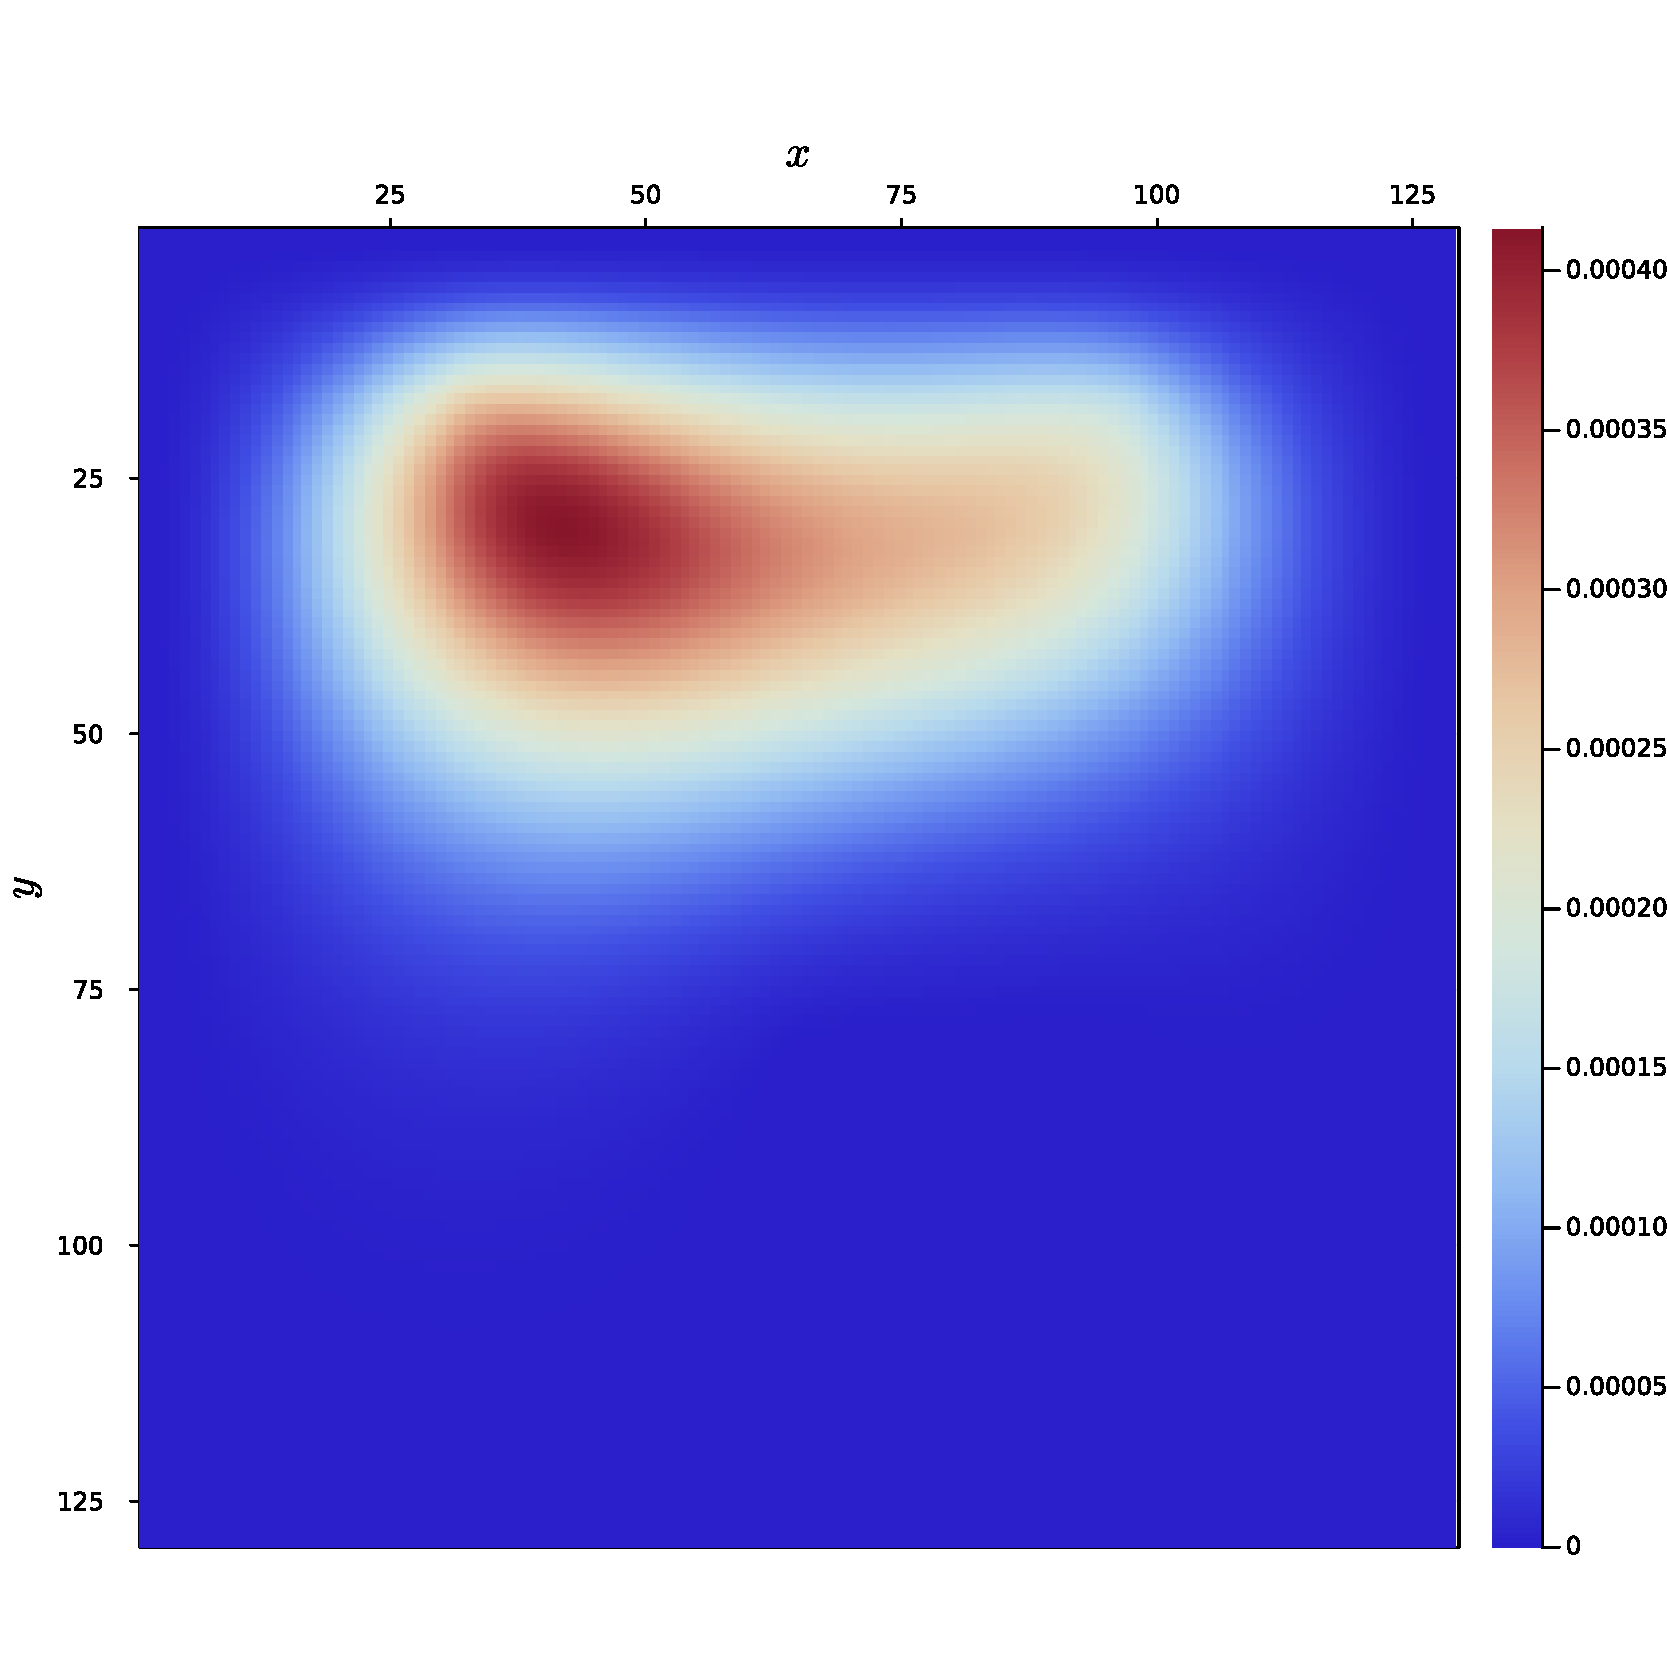
\includegraphics[width=0.8\textwidth]{P_heatmap}
    \caption{The heatmap of the probability of the charged particle appearing at any
        position within the whole region.}
    \label{fig:P_heatmap}
\end{figure}

\begin{figure}[!hbt]
    \centering
    \includegraphics[width=0.8\textwidth]{P_surface}
    \caption{The surface plot of the probability of the charged particle appearing at any
        position within the whole region. The maximal probability is $4.136 \times 10^{-4}$
        (at the peak).}
    \label{fig:P_surface}
\end{figure}
